\documentclass[../main.tex]{subfiles}
\graphicspath{{\subfix{../imagenes/}}}

\begin{document}

\chapter{Conclusions} \label{chap:conclusions} \info{9-10 páginas}
    

    Discussion about the results obtained and implications in the context of the project, limitations of the proposed system, future work, etc.
    

    \section{Main Implications} \label{conclusions:implications} \info{0.65 pág}

    \section{Limitations of the System} \label{conclusions:limitations} \info{0.5 pág}
    
    \section{Future Work} \label{conclusions:future_work} \info{~2.75 pág}
    % \addcontentsline{toc}{section}{Future Work}

    The following section\dots

    \subsection{
        Implementing new adaptation strategies to the system 
    } \label{conclusions:future_work:adaptation_strategies}\info{0.5 pág}


    \subsection{
        Improving the explainability of the continual learning process 
    } \label{conclusions:future_work:explainability}\info{0.5 pág}

    Anytime a model is trained on a particular dataset, any biases present on that dataset are also introduced to the model. In any high-stakes environment, the researchers who design these models should be aware of the biases present in the data and how they might affect the model's predictions and consider them in the decision-making process.

    Furthermore, this aspect is especially crucial in the healthcare sector, where legislation and ethical guidelines stress the importance of AI systems being transparent \cite{noauthor_ethics_2019,eu_aiact_2023}. Healthcare professionals have the moral and legal obligation to be able to explain the decisions made by the AI systems they use to the relevant stakeholders, and the latter also has the right to know how the decisions that affect them are made.
    
    In that regard, one of the main limitations of the system proposed here is the lack of explainability of the continual learning process, where a model that is designed initially to be as transparent as possible might gradually lose explainability power as it adapts to new data distributions over time.
    
    
    
    Methods such as TRAK \cite{park_trak_2023} have been proposed as a way to improve the explainability of Deep Learning models by providing a way to trace the predictions of a model to individual instances of the training data in a concept known as \textit{data attribution}, which has been proven useful in improving sample selection for active learning approaches \cite{park_trak_2023, holzmuller_framework_2023, liu_influence_2021}.

    \subsection{Adapting the system to run on a federated platform} \label{conclusions:future_work:federated} \info{1.75 pág}

    % \info{1 page}

    Federated learning is the concept of training a model using data from multiple sources without having to share the data itself. This is achieved by training the model on each source separately and combining the results to obtain a final model. This technique is particularly useful in healthcare applications, where data privacy is a significant concern. It allows us to train models on data from multiple sources without having to share the data itself, thus preserving the privacy of the patients \cite{joshi_federated_2022}.
    \todo[inline]{Modify this description and add more details, references \dots}

    Efforts such as \cite{joshi_federated_2022} have demonstrated the benefits and potential of taking a federated learning approach to training machine learning models in the healthcare industry. A future proposal to improve the system presented in this work would be to adapt the current platform to one where the models are trained in a federated fashion.
    
    We would propose a system where each research laboratory trains an instance of a (previously agreed) global model with its own local (private) data and shares the trained weights with a central server. The new platform would be mainly used to perform inference on public data, while each client could have an instance of the annotation frontend and backend, including the active learning framework, running locally to annotate their data. 
    
    The motivation for this comes from the fact that is very difficult to convince partners (even within the same project organization) to share their data. In the healthcare industry, data is considered to be a very valuable asset, with a high cost to obtain and annotate, which is why it is often used as a bargaining chip in negotiations between companies and research organizations \todo{include citation}.

    \todo[inline]{Show a diagram of the proposed federated learning system.}

    \clearpage

    \section{Further Research Directions} \label{conclusions:research_directions} \info{~4.5 pág}

    The following are some of the recent and upcoming research directions in the field of machine learning that we consider to be relevant to the work presented in this thesis.
    
    Unlike the previous section, which focused on the limitations of the proposed system and detailed ideas about how to address or improve them in the immediate future, this section takes a broader view, focusing on gaps in the current state-of-the-art and what might be considered to be the next steps in the field.
    
    The idea is that these directions could used as a starting point for future research (i.e. a Ph.D. thesis) on the topics presented in this thesis, either as a continuation of some of the work here or as a completely new approach to the problem. We make no claims about the feasibility of these ideas but rather present why I consider them to be interesting for further research and/or discussion.


    \subsection{Future directions in Tuberculosis AI Research} \label{conclusions:future_work:tb_ai} \info{<1 pág}
    
    Detection will soon be a solved problem thanks to NAATs (or rather, more of a money problem than a technical one). Thus, the emphasis should be less on CV-based detectors and more to advances in drug discovery, finding new biomarkers, etc. \dots

    \clearpage


    \subsection{Scalable Adaptability through Mixtures of Experts} \label{conclusions:research_directions:moes} \info{1.5 pág}

    Mixture of experts (MoE) systems are a type of ensemble model that combines the predictions of multiple models to obtain a final prediction. The difference between MoEs and other ensemble models is that the predictions of the individual `experts' are combined using a gating function that adapts to the given data point and dynamically determines the weight of each model in the final prediction \cite{chen_towards_2022}.

    MoEs are really powerful systems. They have been shown to be able to learn complex multimodal distributions and have been used in a wide variety of applications, including object detection, language modeling, machine translation, and even multiomics \cite{hwang_tutel_2023,mustafa_multimodal_2022,shazeer_outrageously_2017, minoura_scmm_2021}.
    
    But by far, the biggest advantage of MoEs is that each expert model can be deployed independently, allowing for a more flexible, modular system capable of being distributed and data-parallelized among different hardware resources. 

    The computational sparsity of these systems has shown the capacity of MoEs to scale DNN models to outrageous amounts of parameters. Recently, researchers at Google Brain presented a MoE architecture called Switch Transformers \cite{fedusSwitchTransformersScaling2022a} that allows language models - AI systems that can generate text - to scale to even a trillion parameters at a constant computational cost.
    
    Furthermore, systems that take advantage of MoEs to scale LLMs (Large Language Models) already exist and have been deployed to production for applications as big as ChatGPT (GPT-4 is thought to be a MoE with over 8-billion parameters \todo{add citation}).
    
    In the context of the area of this work, we consider that MoEs could be used to create a more scalable and robust system that can adapt to new tasks and data distributions. The idea is that the system would be composed of a set of `expert' models, each of which would be specialized in a particular aspect of the input data. The system would then be able to adapt to new tasks by autonomously learning a new expert model or by retraining an existing one when the need arises.
    
    The main advantage of this approach is that it would allow the system to scale to a large number of tasks and data distributions, only needing to retrain the gating function continually instead of entire models. 
    
    Another advantage is the potential for more failsafe systems. By having each model deployed independently in a distributed system, one could devise a mechanism that detects when one of the expert models fails, either due to a hardware/software error or due to a significant performance drop, and automatically replaces the gating function of the current MoE with one (previously trained) that excludes the failing model.
    
    One could also use such a mechanism as a way to save operational costs. The system might monitor the number of instances being routed to each expert model, and if one of the models is not being used, it could be automatically shut down to save resources.

    Figure \ref{fig:moes} shows a diagram illustrating the concept of a mixture of experts system.

    \begin{figure}[H]
        \centering
        \caption{Diagram of a mixture of experts model.}
        \resizebox*{0.8\linewidth}{!}{
            

\tikzset{every picture/.style={line width=0.75pt}} %set default line width to 0.75pt        

\begin{tikzpicture}[x=0.75pt,y=0.75pt,yscale=-1,xscale=1]
%uncomment if require: \path (0,461); %set diagram left start at 0, and has a height of 461

%Rounded Rect [id:dp4473657659258059] 
\draw  [fill={rgb, 255:red, 80; green, 227; blue, 194 }  ,fill opacity=0.68 ][dash pattern={on 4.5pt off 4.5pt}] (357.54,103.02) .. controls (357.54,88.32) and (369.46,76.4) .. (384.16,76.4) -- (464.03,76.4) .. controls (478.73,76.4) and (490.65,88.32) .. (490.65,103.02) -- (490.65,399.58) .. controls (490.65,414.28) and (478.73,426.2) .. (464.03,426.2) -- (384.16,426.2) .. controls (369.46,426.2) and (357.54,414.28) .. (357.54,399.58) -- cycle ;
%Image [id:dp8982524549343145] 
\draw (61.1,120.57) node  {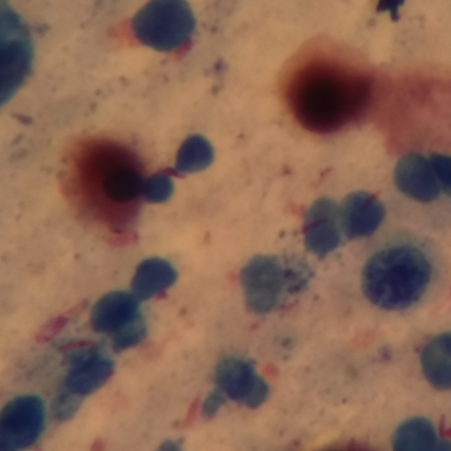
\includegraphics[width=40pt,height=35.05pt]{sputum_smear.png}};
%Curve Lines [id:da6930104671558202] 
\draw    (283.87,225.64) .. controls (287.88,227.01) and (277.93,302.9) .. (355.37,293.48) ;
\draw [shift={(356.55,293.33)}, rotate = 172.52] [color={rgb, 255:red, 0; green, 0; blue, 0 }  ][line width=0.75]    (10.93,-3.29) .. controls (6.95,-1.4) and (3.31,-0.3) .. (0,0) .. controls (3.31,0.3) and (6.95,1.4) .. (10.93,3.29)   ;
%Shape: Ellipse [id:dp08665994720437631] 
\draw  [fill={rgb, 255:red, 245; green, 166; blue, 35 }  ,fill opacity=0.61 ][line width=0.75]  (430.46,108.94) .. controls (430.46,105.03) and (433.55,101.86) .. (437.37,101.86) .. controls (441.19,101.86) and (444.28,105.03) .. (444.28,108.94) .. controls (444.28,112.85) and (441.19,116.03) .. (437.37,116.03) .. controls (433.55,116.03) and (430.46,112.85) .. (430.46,108.94) -- cycle ;
%Shape: Ellipse [id:dp6997855090348835] 
\draw  [fill={rgb, 255:red, 245; green, 166; blue, 35 }  ,fill opacity=0.61 ][line width=0.75]  (430.46,129.19) .. controls (430.46,125.28) and (433.55,122.11) .. (437.37,122.11) .. controls (441.19,122.11) and (444.28,125.28) .. (444.28,129.19) .. controls (444.28,133.1) and (441.19,136.27) .. (437.37,136.27) .. controls (433.55,136.27) and (430.46,133.1) .. (430.46,129.19) -- cycle ;
%Shape: Ellipse [id:dp6691849298178645] 
\draw  [fill={rgb, 255:red, 245; green, 166; blue, 35 }  ,fill opacity=0.61 ][line width=0.75]  (430.83,149.6) .. controls (430.83,145.9) and (433.76,142.9) .. (437.37,142.9) .. controls (440.98,142.9) and (443.91,145.9) .. (443.91,149.6) .. controls (443.91,153.3) and (440.98,156.3) .. (437.37,156.3) .. controls (433.76,156.3) and (430.83,153.3) .. (430.83,149.6) -- cycle ;
%Straight Lines [id:da3527655909497591] 
\draw [fill={rgb, 255:red, 245; green, 166; blue, 35 }  ,fill opacity=0.61 ][line width=0.75]    (369.37,99.96) -- (381.73,100.17) ;
\draw [shift={(383.73,100.2)}, rotate = 180.97] [color={rgb, 255:red, 0; green, 0; blue, 0 }  ][line width=0.75]    (10.93,-3.29) .. controls (6.95,-1.4) and (3.31,-0.3) .. (0,0) .. controls (3.31,0.3) and (6.95,1.4) .. (10.93,3.29)   ;
%Shape: Ellipse [id:dp9370471382922445] 
\draw  [fill={rgb, 255:red, 245; green, 166; blue, 35 }  ,fill opacity=0.61 ][line width=0.75]  (383.73,100.2) .. controls (383.73,96.42) and (386.73,93.34) .. (390.42,93.34) .. controls (394.12,93.34) and (397.12,96.42) .. (397.12,100.2) .. controls (397.12,103.99) and (394.12,107.06) .. (390.42,107.06) .. controls (386.73,107.06) and (383.73,103.99) .. (383.73,100.2) -- cycle ;
%Shape: Ellipse [id:dp20427399962430082] 
\draw  [fill={rgb, 255:red, 245; green, 166; blue, 35 }  ,fill opacity=0.61 ][line width=0.75]  (383.73,119.69) .. controls (383.73,115.78) and (386.82,112.61) .. (390.64,112.61) .. controls (394.46,112.61) and (397.55,115.78) .. (397.55,119.69) .. controls (397.55,123.6) and (394.46,126.77) .. (390.64,126.77) .. controls (386.82,126.77) and (383.73,123.6) .. (383.73,119.69) -- cycle ;
%Shape: Ellipse [id:dp24366723270494473] 
\draw  [fill={rgb, 255:red, 245; green, 166; blue, 35 }  ,fill opacity=0.61 ][line width=0.75]  (383.73,138.2) .. controls (383.73,134.5) and (386.66,131.5) .. (390.27,131.5) .. controls (393.88,131.5) and (396.81,134.5) .. (396.81,138.2) .. controls (396.81,141.9) and (393.88,144.91) .. (390.27,144.91) .. controls (386.66,144.91) and (383.73,141.9) .. (383.73,138.2) -- cycle ;
%Shape: Ellipse [id:dp007626300605791059] 
\draw  [fill={rgb, 255:red, 245; green, 166; blue, 35 }  ,fill opacity=0.61 ][line width=0.75]  (383.36,157.58) .. controls (383.36,153.67) and (386.45,150.5) .. (390.27,150.5) .. controls (394.09,150.5) and (397.18,153.67) .. (397.18,157.58) .. controls (397.18,161.49) and (394.09,164.66) .. (390.27,164.66) .. controls (386.45,164.66) and (383.36,161.49) .. (383.36,157.58) -- cycle ;
%Shape: Ellipse [id:dp22462654396447657] 
\draw  [fill={rgb, 255:red, 245; green, 166; blue, 35 }  ,fill opacity=0.61 ][line width=0.75]  (464.46,129.45) .. controls (464.46,125.54) and (467.55,122.37) .. (471.37,122.37) .. controls (475.19,122.37) and (478.28,125.54) .. (478.28,129.45) .. controls (478.28,133.36) and (475.19,136.53) .. (471.37,136.53) .. controls (467.55,136.53) and (464.46,133.36) .. (464.46,129.45) -- cycle ;
%Straight Lines [id:da31741194855403143] 
\draw [fill={rgb, 255:red, 245; green, 166; blue, 35 }  ,fill opacity=0.61 ][line width=0.75]    (369,157.34) -- (381.36,157.55) ;
\draw [shift={(383.36,157.58)}, rotate = 180.97] [color={rgb, 255:red, 0; green, 0; blue, 0 }  ][line width=0.75]    (10.93,-3.29) .. controls (6.95,-1.4) and (3.31,-0.3) .. (0,0) .. controls (3.31,0.3) and (6.95,1.4) .. (10.93,3.29)   ;
%Straight Lines [id:da557918178883976] 
\draw [fill={rgb, 255:red, 245; green, 166; blue, 35 }  ,fill opacity=0.61 ][line width=0.75]    (397.12,100.2) -- (428.14,106.23) ;
\draw [shift={(431.08,106.8)}, rotate = 190.99] [fill={rgb, 255:red, 0; green, 0; blue, 0 }  ][line width=0.08]  [draw opacity=0] (8.93,-4.29) -- (0,0) -- (8.93,4.29) -- cycle    ;
%Straight Lines [id:da8298879639219123] 
\draw [fill={rgb, 255:red, 245; green, 166; blue, 35 }  ,fill opacity=0.61 ][line width=0.75]    (369.37,119.45) -- (381.73,119.65) ;
\draw [shift={(383.73,119.69)}, rotate = 180.97] [color={rgb, 255:red, 0; green, 0; blue, 0 }  ][line width=0.75]    (10.93,-3.29) .. controls (6.95,-1.4) and (3.31,-0.3) .. (0,0) .. controls (3.31,0.3) and (6.95,1.4) .. (10.93,3.29)   ;
%Straight Lines [id:da699643543130879] 
\draw [fill={rgb, 255:red, 245; green, 166; blue, 35 }  ,fill opacity=0.61 ][line width=0.75]    (369.37,137.96) -- (381.73,138.17) ;
\draw [shift={(383.73,138.2)}, rotate = 180.97] [color={rgb, 255:red, 0; green, 0; blue, 0 }  ][line width=0.75]    (10.93,-3.29) .. controls (6.95,-1.4) and (3.31,-0.3) .. (0,0) .. controls (3.31,0.3) and (6.95,1.4) .. (10.93,3.29)   ;
%Straight Lines [id:da7258143269693516] 
\draw [fill={rgb, 255:red, 245; green, 166; blue, 35 }  ,fill opacity=0.61 ][line width=0.75]    (397.12,100.2) -- (428.71,124.72) ;
\draw [shift={(431.08,126.56)}, rotate = 217.81] [fill={rgb, 255:red, 0; green, 0; blue, 0 }  ][line width=0.08]  [draw opacity=0] (8.93,-4.29) -- (0,0) -- (8.93,4.29) -- cycle    ;
%Straight Lines [id:da6710366760892965] 
\draw [fill={rgb, 255:red, 245; green, 166; blue, 35 }  ,fill opacity=0.61 ][line width=0.75]    (397.12,100.2) -- (430.02,143.92) ;
\draw [shift={(431.82,146.32)}, rotate = 233.04] [fill={rgb, 255:red, 0; green, 0; blue, 0 }  ][line width=0.08]  [draw opacity=0] (8.93,-4.29) -- (0,0) -- (8.93,4.29) -- cycle    ;
%Straight Lines [id:da8663266672527092] 
\draw [fill={rgb, 255:red, 245; green, 166; blue, 35 }  ,fill opacity=0.61 ][line width=0.75]    (397.55,119.69) -- (427.61,109.87) ;
\draw [shift={(430.46,108.94)}, rotate = 161.91] [fill={rgb, 255:red, 0; green, 0; blue, 0 }  ][line width=0.08]  [draw opacity=0] (8.93,-4.29) -- (0,0) -- (8.93,4.29) -- cycle    ;
%Straight Lines [id:da9978546544403384] 
\draw [fill={rgb, 255:red, 245; green, 166; blue, 35 }  ,fill opacity=0.61 ][line width=0.75]    (397.55,119.69) -- (427.58,128.36) ;
\draw [shift={(430.46,129.19)}, rotate = 196.1] [fill={rgb, 255:red, 0; green, 0; blue, 0 }  ][line width=0.08]  [draw opacity=0] (8.93,-4.29) -- (0,0) -- (8.93,4.29) -- cycle    ;
%Straight Lines [id:da9002051077681328] 
\draw [fill={rgb, 255:red, 245; green, 166; blue, 35 }  ,fill opacity=0.61 ][line width=0.75]    (397.55,119.69) -- (428.6,147.6) ;
\draw [shift={(430.83,149.6)}, rotate = 221.95] [fill={rgb, 255:red, 0; green, 0; blue, 0 }  ][line width=0.08]  [draw opacity=0] (8.93,-4.29) -- (0,0) -- (8.93,4.29) -- cycle    ;
%Straight Lines [id:da41111736755966] 
\draw [fill={rgb, 255:red, 245; green, 166; blue, 35 }  ,fill opacity=0.61 ][line width=0.75]    (396.81,138.2) -- (428.3,150.9) ;
\draw [shift={(431.08,152.02)}, rotate = 201.96] [fill={rgb, 255:red, 0; green, 0; blue, 0 }  ][line width=0.08]  [draw opacity=0] (8.93,-4.29) -- (0,0) -- (8.93,4.29) -- cycle    ;
%Straight Lines [id:da8569556866643671] 
\draw [fill={rgb, 255:red, 245; green, 166; blue, 35 }  ,fill opacity=0.61 ][line width=0.75]    (397.18,157.58) -- (429.21,154.23) ;
\draw [shift={(432.19,153.92)}, rotate = 174.03] [fill={rgb, 255:red, 0; green, 0; blue, 0 }  ][line width=0.08]  [draw opacity=0] (8.93,-4.29) -- (0,0) -- (8.93,4.29) -- cycle    ;
%Straight Lines [id:da30256199798058003] 
\draw [fill={rgb, 255:red, 245; green, 166; blue, 35 }  ,fill opacity=0.61 ][line width=0.75]    (396.81,138.2) -- (428.14,131.73) ;
\draw [shift={(431.08,131.12)}, rotate = 168.32] [fill={rgb, 255:red, 0; green, 0; blue, 0 }  ][line width=0.08]  [draw opacity=0] (8.93,-4.29) -- (0,0) -- (8.93,4.29) -- cycle    ;
%Straight Lines [id:da08565074390343796] 
\draw [fill={rgb, 255:red, 245; green, 166; blue, 35 }  ,fill opacity=0.61 ][line width=0.75]    (397.18,157.58) -- (429.36,135.12) ;
\draw [shift={(431.82,133.4)}, rotate = 145.08] [fill={rgb, 255:red, 0; green, 0; blue, 0 }  ][line width=0.08]  [draw opacity=0] (8.93,-4.29) -- (0,0) -- (8.93,4.29) -- cycle    ;
%Straight Lines [id:da633868930331241] 
\draw [fill={rgb, 255:red, 245; green, 166; blue, 35 }  ,fill opacity=0.61 ][line width=0.75]    (397.18,157.58) -- (429.98,115.62) ;
\draw [shift={(431.82,113.26)}, rotate = 128.01] [fill={rgb, 255:red, 0; green, 0; blue, 0 }  ][line width=0.08]  [draw opacity=0] (8.93,-4.29) -- (0,0) -- (8.93,4.29) -- cycle    ;
%Straight Lines [id:da3401355597803415] 
\draw [fill={rgb, 255:red, 245; green, 166; blue, 35 }  ,fill opacity=0.61 ][line width=0.75]    (397.06,138.19) -- (428.74,112.85) ;
\draw [shift={(431.08,110.98)}, rotate = 141.35] [fill={rgb, 255:red, 0; green, 0; blue, 0 }  ][line width=0.08]  [draw opacity=0] (8.93,-4.29) -- (0,0) -- (8.93,4.29) -- cycle    ;
%Straight Lines [id:da8039438988073113] 
\draw [fill={rgb, 255:red, 245; green, 166; blue, 35 }  ,fill opacity=0.61 ][line width=0.75]    (444.28,108.94) -- (465.26,122.15) ;
\draw [shift={(467.8,123.75)}, rotate = 212.2] [fill={rgb, 255:red, 0; green, 0; blue, 0 }  ][line width=0.08]  [draw opacity=0] (8.93,-4.29) -- (0,0) -- (8.93,4.29) -- cycle    ;
%Straight Lines [id:da08826190804441536] 
\draw [fill={rgb, 255:red, 245; green, 166; blue, 35 }  ,fill opacity=0.61 ][line width=0.75]    (444.28,129.19) -- (461.46,129.41) ;
\draw [shift={(464.46,129.45)}, rotate = 180.74] [fill={rgb, 255:red, 0; green, 0; blue, 0 }  ][line width=0.08]  [draw opacity=0] (8.93,-4.29) -- (0,0) -- (8.93,4.29) -- cycle    ;
%Straight Lines [id:da6016749447737926] 
\draw [fill={rgb, 255:red, 245; green, 166; blue, 35 }  ,fill opacity=0.61 ][line width=0.75]    (443.91,149.6) -- (464.55,136.04) ;
\draw [shift={(467.06,134.39)}, rotate = 146.68] [fill={rgb, 255:red, 0; green, 0; blue, 0 }  ][line width=0.08]  [draw opacity=0] (8.93,-4.29) -- (0,0) -- (8.93,4.29) -- cycle    ;

%Shape: Ellipse [id:dp43855366801692974] 
\draw  [fill={rgb, 255:red, 245; green, 166; blue, 35 }  ,fill opacity=0.8 ][line width=0.75]  (431.37,195.07) .. controls (431.37,191.16) and (434.47,187.98) .. (438.29,187.98) .. controls (442.1,187.98) and (445.2,191.16) .. (445.2,195.07) .. controls (445.2,198.98) and (442.1,202.15) .. (438.29,202.15) .. controls (434.47,202.15) and (431.37,198.98) .. (431.37,195.07) -- cycle ;
%Shape: Ellipse [id:dp13853948919551096] 
\draw  [fill={rgb, 255:red, 245; green, 166; blue, 35 }  ,fill opacity=0.8 ][line width=0.75]  (431.37,215.31) .. controls (431.37,211.4) and (434.47,208.23) .. (438.29,208.23) .. controls (442.1,208.23) and (445.2,211.4) .. (445.2,215.31) .. controls (445.2,219.22) and (442.1,222.39) .. (438.29,222.39) .. controls (434.47,222.39) and (431.37,219.22) .. (431.37,215.31) -- cycle ;
%Shape: Ellipse [id:dp7516267985791654] 
\draw  [fill={rgb, 255:red, 245; green, 166; blue, 35 }  ,fill opacity=0.8 ][line width=0.75]  (431.74,235.73) .. controls (431.74,232.02) and (434.67,229.02) .. (438.29,229.02) .. controls (441.9,229.02) and (444.83,232.02) .. (444.83,235.73) .. controls (444.83,239.43) and (441.9,242.43) .. (438.29,242.43) .. controls (434.67,242.43) and (431.74,239.43) .. (431.74,235.73) -- cycle ;
%Straight Lines [id:da14110312192300944] 
\draw [fill={rgb, 255:red, 245; green, 166; blue, 35 }  ,fill opacity=0.8 ][line width=0.75]    (370.28,186.08) -- (382.64,186.29) ;
\draw [shift={(384.64,186.33)}, rotate = 180.97] [color={rgb, 255:red, 0; green, 0; blue, 0 }  ][line width=0.75]    (10.93,-3.29) .. controls (6.95,-1.4) and (3.31,-0.3) .. (0,0) .. controls (3.31,0.3) and (6.95,1.4) .. (10.93,3.29)   ;
%Shape: Ellipse [id:dp5105737926229232] 
\draw  [fill={rgb, 255:red, 245; green, 166; blue, 35 }  ,fill opacity=0.8 ][line width=0.75]  (384.64,186.33) .. controls (384.64,182.54) and (387.64,179.47) .. (391.34,179.47) .. controls (395.03,179.47) and (398.03,182.54) .. (398.03,186.33) .. controls (398.03,190.12) and (395.03,193.19) .. (391.34,193.19) .. controls (387.64,193.19) and (384.64,190.12) .. (384.64,186.33) -- cycle ;
%Shape: Ellipse [id:dp8622935386751234] 
\draw  [fill={rgb, 255:red, 245; green, 166; blue, 35 }  ,fill opacity=0.8 ][line width=0.75]  (384.64,205.81) .. controls (384.64,201.9) and (387.74,198.73) .. (391.56,198.73) .. controls (395.37,198.73) and (398.47,201.9) .. (398.47,205.81) .. controls (398.47,209.72) and (395.37,212.9) .. (391.56,212.9) .. controls (387.74,212.9) and (384.64,209.72) .. (384.64,205.81) -- cycle ;
%Shape: Ellipse [id:dp7175798312397521] 
\draw  [fill={rgb, 255:red, 245; green, 166; blue, 35 }  ,fill opacity=0.8 ][line width=0.75]  (384.64,224.33) .. controls (384.64,220.62) and (387.57,217.62) .. (391.19,217.62) .. controls (394.8,217.62) and (397.73,220.62) .. (397.73,224.33) .. controls (397.73,228.03) and (394.8,231.03) .. (391.19,231.03) .. controls (387.57,231.03) and (384.64,228.03) .. (384.64,224.33) -- cycle ;
%Shape: Ellipse [id:dp28279985646381633] 
\draw  [fill={rgb, 255:red, 245; green, 166; blue, 35 }  ,fill opacity=0.8 ][line width=0.75]  (384.27,243.71) .. controls (384.27,239.79) and (387.37,236.62) .. (391.19,236.62) .. controls (395,236.62) and (398.1,239.79) .. (398.1,243.71) .. controls (398.1,247.62) and (395,250.79) .. (391.19,250.79) .. controls (387.37,250.79) and (384.27,247.62) .. (384.27,243.71) -- cycle ;
%Shape: Ellipse [id:dp475505176196914] 
\draw  [fill={rgb, 255:red, 245; green, 166; blue, 35 }  ,fill opacity=0.8 ][line width=0.75]  (465.37,215.57) .. controls (465.37,211.66) and (468.47,208.49) .. (472.29,208.49) .. controls (476.11,208.49) and (479.2,211.66) .. (479.2,215.57) .. controls (479.2,219.48) and (476.11,222.65) .. (472.29,222.65) .. controls (468.47,222.65) and (465.37,219.48) .. (465.37,215.57) -- cycle ;
%Straight Lines [id:da0880468074847438] 
\draw [fill={rgb, 255:red, 245; green, 166; blue, 35 }  ,fill opacity=0.8 ][line width=0.75]    (369.91,243.46) -- (382.27,243.67) ;
\draw [shift={(384.27,243.71)}, rotate = 180.97] [color={rgb, 255:red, 0; green, 0; blue, 0 }  ][line width=0.75]    (10.93,-3.29) .. controls (6.95,-1.4) and (3.31,-0.3) .. (0,0) .. controls (3.31,0.3) and (6.95,1.4) .. (10.93,3.29)   ;
%Straight Lines [id:da4973999338201691] 
\draw [fill={rgb, 255:red, 245; green, 166; blue, 35 }  ,fill opacity=0.8 ][line width=0.75]    (398.03,186.33) -- (429.05,192.35) ;
\draw [shift={(432,192.92)}, rotate = 190.99] [fill={rgb, 255:red, 0; green, 0; blue, 0 }  ][line width=0.08]  [draw opacity=0] (8.93,-4.29) -- (0,0) -- (8.93,4.29) -- cycle    ;
%Straight Lines [id:da806322175872451] 
\draw [fill={rgb, 255:red, 245; green, 166; blue, 35 }  ,fill opacity=0.8 ][line width=0.75]    (370.28,205.57) -- (382.64,205.78) ;
\draw [shift={(384.64,205.81)}, rotate = 180.97] [color={rgb, 255:red, 0; green, 0; blue, 0 }  ][line width=0.75]    (10.93,-3.29) .. controls (6.95,-1.4) and (3.31,-0.3) .. (0,0) .. controls (3.31,0.3) and (6.95,1.4) .. (10.93,3.29)   ;
%Straight Lines [id:da7276134544408976] 
\draw [fill={rgb, 255:red, 245; green, 166; blue, 35 }  ,fill opacity=0.8 ][line width=0.75]    (370.28,224.08) -- (382.64,224.29) ;
\draw [shift={(384.64,224.33)}, rotate = 180.97] [color={rgb, 255:red, 0; green, 0; blue, 0 }  ][line width=0.75]    (10.93,-3.29) .. controls (6.95,-1.4) and (3.31,-0.3) .. (0,0) .. controls (3.31,0.3) and (6.95,1.4) .. (10.93,3.29)   ;
%Straight Lines [id:da8489045712598526] 
\draw [fill={rgb, 255:red, 245; green, 166; blue, 35 }  ,fill opacity=0.8 ][line width=0.75]    (398.03,186.33) -- (429.63,210.84) ;
\draw [shift={(432,212.68)}, rotate = 217.81] [fill={rgb, 255:red, 0; green, 0; blue, 0 }  ][line width=0.08]  [draw opacity=0] (8.93,-4.29) -- (0,0) -- (8.93,4.29) -- cycle    ;
%Straight Lines [id:da013293072789012594] 
\draw [fill={rgb, 255:red, 245; green, 166; blue, 35 }  ,fill opacity=0.8 ][line width=0.75]    (398.03,186.33) -- (430.93,230.05) ;
\draw [shift={(432.74,232.44)}, rotate = 233.04] [fill={rgb, 255:red, 0; green, 0; blue, 0 }  ][line width=0.08]  [draw opacity=0] (8.93,-4.29) -- (0,0) -- (8.93,4.29) -- cycle    ;
%Straight Lines [id:da38754352601338793] 
\draw [fill={rgb, 255:red, 245; green, 166; blue, 35 }  ,fill opacity=0.8 ][line width=0.75]    (398.47,205.81) -- (428.52,196) ;
\draw [shift={(431.37,195.07)}, rotate = 161.91] [fill={rgb, 255:red, 0; green, 0; blue, 0 }  ][line width=0.08]  [draw opacity=0] (8.93,-4.29) -- (0,0) -- (8.93,4.29) -- cycle    ;
%Straight Lines [id:da7655831145463079] 
\draw [fill={rgb, 255:red, 245; green, 166; blue, 35 }  ,fill opacity=0.8 ][line width=0.75]    (398.47,205.81) -- (428.49,214.48) ;
\draw [shift={(431.37,215.31)}, rotate = 196.1] [fill={rgb, 255:red, 0; green, 0; blue, 0 }  ][line width=0.08]  [draw opacity=0] (8.93,-4.29) -- (0,0) -- (8.93,4.29) -- cycle    ;
%Straight Lines [id:da10372540088180715] 
\draw [fill={rgb, 255:red, 245; green, 166; blue, 35 }  ,fill opacity=0.8 ][line width=0.75]    (398.47,205.81) -- (429.51,233.72) ;
\draw [shift={(431.74,235.73)}, rotate = 221.95] [fill={rgb, 255:red, 0; green, 0; blue, 0 }  ][line width=0.08]  [draw opacity=0] (8.93,-4.29) -- (0,0) -- (8.93,4.29) -- cycle    ;
%Straight Lines [id:da15602052141985778] 
\draw [fill={rgb, 255:red, 245; green, 166; blue, 35 }  ,fill opacity=0.8 ][line width=0.75]    (397.73,224.33) -- (429.21,237.02) ;
\draw [shift={(432,238.14)}, rotate = 201.96] [fill={rgb, 255:red, 0; green, 0; blue, 0 }  ][line width=0.08]  [draw opacity=0] (8.93,-4.29) -- (0,0) -- (8.93,4.29) -- cycle    ;
%Straight Lines [id:da5819168880222307] 
\draw [fill={rgb, 255:red, 245; green, 166; blue, 35 }  ,fill opacity=0.8 ][line width=0.75]    (398.1,243.71) -- (430.12,240.35) ;
\draw [shift={(433.11,240.04)}, rotate = 174.03] [fill={rgb, 255:red, 0; green, 0; blue, 0 }  ][line width=0.08]  [draw opacity=0] (8.93,-4.29) -- (0,0) -- (8.93,4.29) -- cycle    ;
%Straight Lines [id:da7935569845988224] 
\draw [fill={rgb, 255:red, 245; green, 166; blue, 35 }  ,fill opacity=0.8 ][line width=0.75]    (397.73,224.33) -- (429.06,217.85) ;
\draw [shift={(432,217.24)}, rotate = 168.32] [fill={rgb, 255:red, 0; green, 0; blue, 0 }  ][line width=0.08]  [draw opacity=0] (8.93,-4.29) -- (0,0) -- (8.93,4.29) -- cycle    ;
%Straight Lines [id:da21492152328433645] 
\draw [fill={rgb, 255:red, 245; green, 166; blue, 35 }  ,fill opacity=0.8 ][line width=0.75]    (398.1,243.71) -- (430.28,221.24) ;
\draw [shift={(432.74,219.52)}, rotate = 145.08] [fill={rgb, 255:red, 0; green, 0; blue, 0 }  ][line width=0.08]  [draw opacity=0] (8.93,-4.29) -- (0,0) -- (8.93,4.29) -- cycle    ;
%Straight Lines [id:da4847658277621407] 
\draw [fill={rgb, 255:red, 245; green, 166; blue, 35 }  ,fill opacity=0.8 ][line width=0.75]    (398.1,243.71) -- (430.89,201.75) ;
\draw [shift={(432.74,199.38)}, rotate = 128.01] [fill={rgb, 255:red, 0; green, 0; blue, 0 }  ][line width=0.08]  [draw opacity=0] (8.93,-4.29) -- (0,0) -- (8.93,4.29) -- cycle    ;
%Straight Lines [id:da37701120023744794] 
\draw [fill={rgb, 255:red, 245; green, 166; blue, 35 }  ,fill opacity=0.8 ][line width=0.75]    (397.97,224.31) -- (429.65,198.98) ;
\draw [shift={(432,197.1)}, rotate = 141.35] [fill={rgb, 255:red, 0; green, 0; blue, 0 }  ][line width=0.08]  [draw opacity=0] (8.93,-4.29) -- (0,0) -- (8.93,4.29) -- cycle    ;
%Straight Lines [id:da645561066385429] 
\draw [fill={rgb, 255:red, 245; green, 166; blue, 35 }  ,fill opacity=0.8 ][line width=0.75]    (445.2,195.07) -- (466.17,208.27) ;
\draw [shift={(468.71,209.87)}, rotate = 212.2] [fill={rgb, 255:red, 0; green, 0; blue, 0 }  ][line width=0.08]  [draw opacity=0] (8.93,-4.29) -- (0,0) -- (8.93,4.29) -- cycle    ;
%Straight Lines [id:da38124151730490485] 
\draw [fill={rgb, 255:red, 245; green, 166; blue, 35 }  ,fill opacity=0.8 ][line width=0.75]    (445.2,215.31) -- (462.37,215.53) ;
\draw [shift={(465.37,215.57)}, rotate = 180.74] [fill={rgb, 255:red, 0; green, 0; blue, 0 }  ][line width=0.08]  [draw opacity=0] (8.93,-4.29) -- (0,0) -- (8.93,4.29) -- cycle    ;
%Straight Lines [id:da940145278566491] 
\draw [fill={rgb, 255:red, 245; green, 166; blue, 35 }  ,fill opacity=0.8 ][line width=0.75]    (444.83,235.73) -- (465.46,222.16) ;
\draw [shift={(467.97,220.51)}, rotate = 146.68] [fill={rgb, 255:red, 0; green, 0; blue, 0 }  ][line width=0.08]  [draw opacity=0] (8.93,-4.29) -- (0,0) -- (8.93,4.29) -- cycle    ;

%Shape: Ellipse [id:dp1488873719978694] 
\draw  [line width=0.75]  (428.63,278.61) .. controls (428.63,274.7) and (431.72,271.52) .. (435.54,271.52) .. controls (439.36,271.52) and (442.45,274.7) .. (442.45,278.61) .. controls (442.45,282.52) and (439.36,285.69) .. (435.54,285.69) .. controls (431.72,285.69) and (428.63,282.52) .. (428.63,278.61) -- cycle ;
%Shape: Ellipse [id:dp45983770948179004] 
\draw  [line width=0.75]  (428.63,298.85) .. controls (428.63,294.94) and (431.72,291.77) .. (435.54,291.77) .. controls (439.36,291.77) and (442.45,294.94) .. (442.45,298.85) .. controls (442.45,302.76) and (439.36,305.93) .. (435.54,305.93) .. controls (431.72,305.93) and (428.63,302.76) .. (428.63,298.85) -- cycle ;
%Shape: Ellipse [id:dp42685940811514] 
\draw  [line width=0.75]  (429,319.27) .. controls (429,315.56) and (431.93,312.56) .. (435.54,312.56) .. controls (439.15,312.56) and (442.08,315.56) .. (442.08,319.27) .. controls (442.08,322.97) and (439.15,325.97) .. (435.54,325.97) .. controls (431.93,325.97) and (429,322.97) .. (429,319.27) -- cycle ;
%Straight Lines [id:da143820194586048] 
\draw [line width=0.75]    (367.54,269.62) -- (379.9,269.83) ;
\draw [shift={(381.9,269.87)}, rotate = 180.97] [color={rgb, 255:red, 0; green, 0; blue, 0 }  ][line width=0.75]    (10.93,-3.29) .. controls (6.95,-1.4) and (3.31,-0.3) .. (0,0) .. controls (3.31,0.3) and (6.95,1.4) .. (10.93,3.29)   ;
%Shape: Ellipse [id:dp5140351997691064] 
\draw  [line width=0.75]  (381.9,269.87) .. controls (381.9,266.08) and (384.89,263.01) .. (388.59,263.01) .. controls (392.29,263.01) and (395.29,266.08) .. (395.29,269.87) .. controls (395.29,273.66) and (392.29,276.73) .. (388.59,276.73) .. controls (384.89,276.73) and (381.9,273.66) .. (381.9,269.87) -- cycle ;
%Shape: Ellipse [id:dp25662349488432046] 
\draw  [line width=0.75]  (381.9,289.35) .. controls (381.9,285.44) and (384.99,282.27) .. (388.81,282.27) .. controls (392.63,282.27) and (395.72,285.44) .. (395.72,289.35) .. controls (395.72,293.26) and (392.63,296.43) .. (388.81,296.43) .. controls (384.99,296.43) and (381.9,293.26) .. (381.9,289.35) -- cycle ;
%Shape: Ellipse [id:dp252271951498815] 
\draw  [line width=0.75]  (381.9,307.87) .. controls (381.9,304.16) and (384.83,301.16) .. (388.44,301.16) .. controls (392.05,301.16) and (394.98,304.16) .. (394.98,307.87) .. controls (394.98,311.57) and (392.05,314.57) .. (388.44,314.57) .. controls (384.83,314.57) and (381.9,311.57) .. (381.9,307.87) -- cycle ;
%Shape: Ellipse [id:dp938255899162866] 
\draw  [line width=0.75]  (381.53,327.25) .. controls (381.53,323.33) and (384.62,320.16) .. (388.44,320.16) .. controls (392.26,320.16) and (395.35,323.33) .. (395.35,327.25) .. controls (395.35,331.16) and (392.26,334.33) .. (388.44,334.33) .. controls (384.62,334.33) and (381.53,331.16) .. (381.53,327.25) -- cycle ;
%Shape: Ellipse [id:dp6670913819174638] 
\draw  [line width=0.75]  (462.63,299.11) .. controls (462.63,295.2) and (465.72,292.03) .. (469.54,292.03) .. controls (473.36,292.03) and (476.45,295.2) .. (476.45,299.11) .. controls (476.45,303.02) and (473.36,306.19) .. (469.54,306.19) .. controls (465.72,306.19) and (462.63,303.02) .. (462.63,299.11) -- cycle ;
%Straight Lines [id:da4116763116703259] 
\draw [line width=0.75]    (367.17,327) -- (379.53,327.21) ;
\draw [shift={(381.53,327.25)}, rotate = 180.97] [color={rgb, 255:red, 0; green, 0; blue, 0 }  ][line width=0.75]    (10.93,-3.29) .. controls (6.95,-1.4) and (3.31,-0.3) .. (0,0) .. controls (3.31,0.3) and (6.95,1.4) .. (10.93,3.29)   ;
%Straight Lines [id:da6544592847055477] 
\draw [line width=0.75]    (395.29,269.87) -- (426.31,275.89) ;
\draw [shift={(429.25,276.46)}, rotate = 190.99] [fill={rgb, 255:red, 0; green, 0; blue, 0 }  ][line width=0.08]  [draw opacity=0] (8.93,-4.29) -- (0,0) -- (8.93,4.29) -- cycle    ;
%Straight Lines [id:da8983357153193312] 
\draw [line width=0.75]    (367.54,289.11) -- (379.9,289.32) ;
\draw [shift={(381.9,289.35)}, rotate = 180.97] [color={rgb, 255:red, 0; green, 0; blue, 0 }  ][line width=0.75]    (10.93,-3.29) .. controls (6.95,-1.4) and (3.31,-0.3) .. (0,0) .. controls (3.31,0.3) and (6.95,1.4) .. (10.93,3.29)   ;
%Straight Lines [id:da4331749885302525] 
\draw [line width=0.75]    (367.54,307.62) -- (379.9,307.83) ;
\draw [shift={(381.9,307.87)}, rotate = 180.97] [color={rgb, 255:red, 0; green, 0; blue, 0 }  ][line width=0.75]    (10.93,-3.29) .. controls (6.95,-1.4) and (3.31,-0.3) .. (0,0) .. controls (3.31,0.3) and (6.95,1.4) .. (10.93,3.29)   ;
%Straight Lines [id:da8645896121308936] 
\draw [line width=0.75]    (395.29,269.87) -- (426.88,294.38) ;
\draw [shift={(429.25,296.22)}, rotate = 217.81] [fill={rgb, 255:red, 0; green, 0; blue, 0 }  ][line width=0.08]  [draw opacity=0] (8.93,-4.29) -- (0,0) -- (8.93,4.29) -- cycle    ;
%Straight Lines [id:da9028915560676274] 
\draw [line width=0.75]    (395.29,269.87) -- (428.19,313.59) ;
\draw [shift={(429.99,315.98)}, rotate = 233.04] [fill={rgb, 255:red, 0; green, 0; blue, 0 }  ][line width=0.08]  [draw opacity=0] (8.93,-4.29) -- (0,0) -- (8.93,4.29) -- cycle    ;
%Straight Lines [id:da47812405231539046] 
\draw [line width=0.75]    (395.72,289.35) -- (425.78,279.54) ;
\draw [shift={(428.63,278.61)}, rotate = 161.91] [fill={rgb, 255:red, 0; green, 0; blue, 0 }  ][line width=0.08]  [draw opacity=0] (8.93,-4.29) -- (0,0) -- (8.93,4.29) -- cycle    ;
%Straight Lines [id:da03723604455754326] 
\draw [line width=0.75]    (395.72,289.35) -- (425.75,298.02) ;
\draw [shift={(428.63,298.85)}, rotate = 196.1] [fill={rgb, 255:red, 0; green, 0; blue, 0 }  ][line width=0.08]  [draw opacity=0] (8.93,-4.29) -- (0,0) -- (8.93,4.29) -- cycle    ;
%Straight Lines [id:da046384628953082485] 
\draw [line width=0.75]    (395.72,289.35) -- (426.77,317.26) ;
\draw [shift={(429,319.27)}, rotate = 221.95] [fill={rgb, 255:red, 0; green, 0; blue, 0 }  ][line width=0.08]  [draw opacity=0] (8.93,-4.29) -- (0,0) -- (8.93,4.29) -- cycle    ;
%Straight Lines [id:da14833225667560668] 
\draw [line width=0.75]    (394.98,307.87) -- (426.47,320.56) ;
\draw [shift={(429.25,321.68)}, rotate = 201.96] [fill={rgb, 255:red, 0; green, 0; blue, 0 }  ][line width=0.08]  [draw opacity=0] (8.93,-4.29) -- (0,0) -- (8.93,4.29) -- cycle    ;
%Straight Lines [id:da8442561408509968] 
\draw [line width=0.75]    (395.35,327.25) -- (427.38,323.89) ;
\draw [shift={(430.36,323.58)}, rotate = 174.03] [fill={rgb, 255:red, 0; green, 0; blue, 0 }  ][line width=0.08]  [draw opacity=0] (8.93,-4.29) -- (0,0) -- (8.93,4.29) -- cycle    ;
%Straight Lines [id:da1236744129269951] 
\draw [line width=0.75]    (394.98,307.87) -- (426.31,301.39) ;
\draw [shift={(429.25,300.78)}, rotate = 168.32] [fill={rgb, 255:red, 0; green, 0; blue, 0 }  ][line width=0.08]  [draw opacity=0] (8.93,-4.29) -- (0,0) -- (8.93,4.29) -- cycle    ;
%Straight Lines [id:da11746166348461529] 
\draw [line width=0.75]    (395.35,327.25) -- (427.53,304.78) ;
\draw [shift={(429.99,303.06)}, rotate = 145.08] [fill={rgb, 255:red, 0; green, 0; blue, 0 }  ][line width=0.08]  [draw opacity=0] (8.93,-4.29) -- (0,0) -- (8.93,4.29) -- cycle    ;
%Straight Lines [id:da40367822672058606] 
\draw [line width=0.75]    (395.35,327.25) -- (428.14,285.29) ;
\draw [shift={(429.99,282.92)}, rotate = 128.01] [fill={rgb, 255:red, 0; green, 0; blue, 0 }  ][line width=0.08]  [draw opacity=0] (8.93,-4.29) -- (0,0) -- (8.93,4.29) -- cycle    ;
%Straight Lines [id:da3775117517837141] 
\draw [line width=0.75]    (395.23,307.85) -- (426.91,282.52) ;
\draw [shift={(429.25,280.64)}, rotate = 141.35] [fill={rgb, 255:red, 0; green, 0; blue, 0 }  ][line width=0.08]  [draw opacity=0] (8.93,-4.29) -- (0,0) -- (8.93,4.29) -- cycle    ;
%Straight Lines [id:da6949233664592245] 
\draw [line width=0.75]    (442.45,278.61) -- (463.43,291.81) ;
\draw [shift={(465.97,293.41)}, rotate = 212.2] [fill={rgb, 255:red, 0; green, 0; blue, 0 }  ][line width=0.08]  [draw opacity=0] (8.93,-4.29) -- (0,0) -- (8.93,4.29) -- cycle    ;
%Straight Lines [id:da3385891355270363] 
\draw [line width=0.75]    (442.45,298.85) -- (459.63,299.07) ;
\draw [shift={(462.63,299.11)}, rotate = 180.74] [fill={rgb, 255:red, 0; green, 0; blue, 0 }  ][line width=0.08]  [draw opacity=0] (8.93,-4.29) -- (0,0) -- (8.93,4.29) -- cycle    ;
%Straight Lines [id:da36911198180647364] 
\draw [line width=0.75]    (442.08,319.27) -- (462.72,305.7) ;
\draw [shift={(465.22,304.05)}, rotate = 146.68] [fill={rgb, 255:red, 0; green, 0; blue, 0 }  ][line width=0.08]  [draw opacity=0] (8.93,-4.29) -- (0,0) -- (8.93,4.29) -- cycle    ;

%Straight Lines [id:da7224011049777017] 
\draw [color={rgb, 255:red, 208; green, 2; blue, 27 }  ,draw opacity=1 ]   (478.28,129.45) -- (549.33,216.85) ;
\draw [shift={(550.59,218.41)}, rotate = 230.89] [color={rgb, 255:red, 208; green, 2; blue, 27 }  ,draw opacity=1 ][line width=0.75]    (10.93,-3.29) .. controls (6.95,-1.4) and (3.31,-0.3) .. (0,0) .. controls (3.31,0.3) and (6.95,1.4) .. (10.93,3.29)   ;
%Straight Lines [id:da3608523285692655] 
\draw [color={rgb, 255:red, 208; green, 2; blue, 27 }  ,draw opacity=1 ]   (479.2,215.57) -- (536.77,231.65) ;
\draw [shift={(538.7,232.19)}, rotate = 195.6] [color={rgb, 255:red, 208; green, 2; blue, 27 }  ,draw opacity=1 ][line width=0.75]    (10.93,-3.29) .. controls (6.95,-1.4) and (3.31,-0.3) .. (0,0) .. controls (3.31,0.3) and (6.95,1.4) .. (10.93,3.29)   ;
%Shape: Ellipse [id:dp8047226865558774] 
\draw  [fill={rgb, 255:red, 126; green, 211; blue, 33 }  ,fill opacity=0.7 ][dash pattern={on 4.5pt off 4.5pt}] (537.41,237.18) .. controls (537.41,225.29) and (547.66,215.65) .. (560.3,215.65) .. controls (572.94,215.65) and (583.18,225.29) .. (583.18,237.18) .. controls (583.18,249.07) and (572.94,258.71) .. (560.3,258.71) .. controls (547.66,258.71) and (537.41,249.07) .. (537.41,237.18) -- cycle ;
%Straight Lines [id:da1748776131536356] 
\draw    (583.18,237.18) -- (605.35,237.65) ;
\draw [shift={(607.34,237.7)}, rotate = 181.23] [color={rgb, 255:red, 0; green, 0; blue, 0 }  ][line width=0.75]    (10.93,-3.29) .. controls (6.95,-1.4) and (3.31,-0.3) .. (0,0) .. controls (3.31,0.3) and (6.95,1.4) .. (10.93,3.29)   ;
%Shape: Ellipse [id:dp7585568424503171] 
\draw  [fill={rgb, 255:red, 245; green, 166; blue, 35 }  ,fill opacity=0.96 ][line width=0.75]  (427.71,356.98) .. controls (427.71,353.07) and (430.81,349.9) .. (434.63,349.9) .. controls (438.44,349.9) and (441.54,353.07) .. (441.54,356.98) .. controls (441.54,360.89) and (438.44,364.06) .. (434.63,364.06) .. controls (430.81,364.06) and (427.71,360.89) .. (427.71,356.98) -- cycle ;
%Shape: Ellipse [id:dp9130085978027553] 
\draw  [fill={rgb, 255:red, 245; green, 166; blue, 35 }  ,fill opacity=0.96 ][line width=0.75]  (427.71,377.22) .. controls (427.71,373.31) and (430.81,370.14) .. (434.63,370.14) .. controls (438.44,370.14) and (441.54,373.31) .. (441.54,377.22) .. controls (441.54,381.14) and (438.44,384.31) .. (434.63,384.31) .. controls (430.81,384.31) and (427.71,381.14) .. (427.71,377.22) -- cycle ;
%Shape: Ellipse [id:dp3906995428530913] 
\draw  [fill={rgb, 255:red, 245; green, 166; blue, 35 }  ,fill opacity=0.96 ][line width=0.75]  (428.08,397.64) .. controls (428.08,393.94) and (431.01,390.94) .. (434.63,390.94) .. controls (438.24,390.94) and (441.17,393.94) .. (441.17,397.64) .. controls (441.17,401.34) and (438.24,404.34) .. (434.63,404.34) .. controls (431.01,404.34) and (428.08,401.34) .. (428.08,397.64) -- cycle ;
%Straight Lines [id:da6265645240651057] 
\draw [fill={rgb, 255:red, 245; green, 166; blue, 35 }  ,fill opacity=0.96 ][line width=0.75]    (366.62,348) -- (378.98,348.21) ;
\draw [shift={(380.98,348.24)}, rotate = 180.97] [color={rgb, 255:red, 0; green, 0; blue, 0 }  ][line width=0.75]    (10.93,-3.29) .. controls (6.95,-1.4) and (3.31,-0.3) .. (0,0) .. controls (3.31,0.3) and (6.95,1.4) .. (10.93,3.29)   ;
%Shape: Ellipse [id:dp8415595381856844] 
\draw  [fill={rgb, 255:red, 245; green, 166; blue, 35 }  ,fill opacity=0.96 ][line width=0.75]  (380.98,348.24) .. controls (380.98,344.45) and (383.98,341.38) .. (387.68,341.38) .. controls (391.37,341.38) and (394.37,344.45) .. (394.37,348.24) .. controls (394.37,352.03) and (391.37,355.1) .. (387.68,355.1) .. controls (383.98,355.1) and (380.98,352.03) .. (380.98,348.24) -- cycle ;
%Shape: Ellipse [id:dp5902790874429655] 
\draw  [fill={rgb, 255:red, 245; green, 166; blue, 35 }  ,fill opacity=0.96 ][line width=0.75]  (380.98,367.72) .. controls (380.98,363.81) and (384.08,360.64) .. (387.89,360.64) .. controls (391.71,360.64) and (394.81,363.81) .. (394.81,367.72) .. controls (394.81,371.64) and (391.71,374.81) .. (387.89,374.81) .. controls (384.08,374.81) and (380.98,371.64) .. (380.98,367.72) -- cycle ;
%Shape: Ellipse [id:dp036178861366020776] 
\draw  [fill={rgb, 255:red, 245; green, 166; blue, 35 }  ,fill opacity=0.96 ][line width=0.75]  (380.98,386.24) .. controls (380.98,382.54) and (383.91,379.54) .. (387.52,379.54) .. controls (391.14,379.54) and (394.07,382.54) .. (394.07,386.24) .. controls (394.07,389.94) and (391.14,392.94) .. (387.52,392.94) .. controls (383.91,392.94) and (380.98,389.94) .. (380.98,386.24) -- cycle ;
%Shape: Ellipse [id:dp6455290592833196] 
\draw  [fill={rgb, 255:red, 245; green, 166; blue, 35 }  ,fill opacity=0.96 ][line width=0.75]  (380.61,405.62) .. controls (380.61,401.71) and (383.71,398.54) .. (387.52,398.54) .. controls (391.34,398.54) and (394.44,401.71) .. (394.44,405.62) .. controls (394.44,409.53) and (391.34,412.7) .. (387.52,412.7) .. controls (383.71,412.7) and (380.61,409.53) .. (380.61,405.62) -- cycle ;
%Shape: Ellipse [id:dp7472810835168311] 
\draw  [fill={rgb, 255:red, 245; green, 166; blue, 35 }  ,fill opacity=0.96 ][line width=0.75]  (461.71,377.48) .. controls (461.71,373.57) and (464.81,370.4) .. (468.63,370.4) .. controls (472.44,370.4) and (475.54,373.57) .. (475.54,377.48) .. controls (475.54,381.4) and (472.44,384.57) .. (468.63,384.57) .. controls (464.81,384.57) and (461.71,381.4) .. (461.71,377.48) -- cycle ;
%Straight Lines [id:da9409496686106043] 
\draw [fill={rgb, 255:red, 245; green, 166; blue, 35 }  ,fill opacity=0.96 ][line width=0.75]    (366.25,405.38) -- (378.61,405.58) ;
\draw [shift={(380.61,405.62)}, rotate = 180.97] [color={rgb, 255:red, 0; green, 0; blue, 0 }  ][line width=0.75]    (10.93,-3.29) .. controls (6.95,-1.4) and (3.31,-0.3) .. (0,0) .. controls (3.31,0.3) and (6.95,1.4) .. (10.93,3.29)   ;
%Straight Lines [id:da29918170125307664] 
\draw [fill={rgb, 255:red, 245; green, 166; blue, 35 }  ,fill opacity=0.96 ][line width=0.75]    (394.37,348.24) -- (425.39,354.26) ;
\draw [shift={(428.33,354.84)}, rotate = 190.99] [fill={rgb, 255:red, 0; green, 0; blue, 0 }  ][line width=0.08]  [draw opacity=0] (8.93,-4.29) -- (0,0) -- (8.93,4.29) -- cycle    ;
%Straight Lines [id:da6218886539599688] 
\draw [fill={rgb, 255:red, 245; green, 166; blue, 35 }  ,fill opacity=0.96 ][line width=0.75]    (366.62,367.48) -- (378.98,367.69) ;
\draw [shift={(380.98,367.72)}, rotate = 180.97] [color={rgb, 255:red, 0; green, 0; blue, 0 }  ][line width=0.75]    (10.93,-3.29) .. controls (6.95,-1.4) and (3.31,-0.3) .. (0,0) .. controls (3.31,0.3) and (6.95,1.4) .. (10.93,3.29)   ;
%Straight Lines [id:da5613633823065742] 
\draw [fill={rgb, 255:red, 245; green, 166; blue, 35 }  ,fill opacity=0.96 ][line width=0.75]    (366.62,386) -- (378.98,386.2) ;
\draw [shift={(380.98,386.24)}, rotate = 180.97] [color={rgb, 255:red, 0; green, 0; blue, 0 }  ][line width=0.75]    (10.93,-3.29) .. controls (6.95,-1.4) and (3.31,-0.3) .. (0,0) .. controls (3.31,0.3) and (6.95,1.4) .. (10.93,3.29)   ;
%Straight Lines [id:da6158697070353689] 
\draw [fill={rgb, 255:red, 245; green, 166; blue, 35 }  ,fill opacity=0.96 ][line width=0.75]    (394.37,348.24) -- (425.96,372.76) ;
\draw [shift={(428.33,374.6)}, rotate = 217.81] [fill={rgb, 255:red, 0; green, 0; blue, 0 }  ][line width=0.08]  [draw opacity=0] (8.93,-4.29) -- (0,0) -- (8.93,4.29) -- cycle    ;
%Straight Lines [id:da26156333876491655] 
\draw [fill={rgb, 255:red, 245; green, 166; blue, 35 }  ,fill opacity=0.96 ][line width=0.75]    (394.37,348.24) -- (427.27,391.96) ;
\draw [shift={(429.08,394.36)}, rotate = 233.04] [fill={rgb, 255:red, 0; green, 0; blue, 0 }  ][line width=0.08]  [draw opacity=0] (8.93,-4.29) -- (0,0) -- (8.93,4.29) -- cycle    ;
%Straight Lines [id:da6533269249420282] 
\draw [fill={rgb, 255:red, 245; green, 166; blue, 35 }  ,fill opacity=0.96 ][line width=0.75]    (394.81,367.72) -- (424.86,357.91) ;
\draw [shift={(427.71,356.98)}, rotate = 161.91] [fill={rgb, 255:red, 0; green, 0; blue, 0 }  ][line width=0.08]  [draw opacity=0] (8.93,-4.29) -- (0,0) -- (8.93,4.29) -- cycle    ;
%Straight Lines [id:da43602198835821815] 
\draw [fill={rgb, 255:red, 245; green, 166; blue, 35 }  ,fill opacity=0.96 ][line width=0.75]    (394.81,367.72) -- (424.83,376.39) ;
\draw [shift={(427.71,377.22)}, rotate = 196.1] [fill={rgb, 255:red, 0; green, 0; blue, 0 }  ][line width=0.08]  [draw opacity=0] (8.93,-4.29) -- (0,0) -- (8.93,4.29) -- cycle    ;
%Straight Lines [id:da57645348985782] 
\draw [fill={rgb, 255:red, 245; green, 166; blue, 35 }  ,fill opacity=0.96 ][line width=0.75]    (394.81,367.72) -- (425.85,395.63) ;
\draw [shift={(428.08,397.64)}, rotate = 221.95] [fill={rgb, 255:red, 0; green, 0; blue, 0 }  ][line width=0.08]  [draw opacity=0] (8.93,-4.29) -- (0,0) -- (8.93,4.29) -- cycle    ;
%Straight Lines [id:da159579614568629] 
\draw [fill={rgb, 255:red, 245; green, 166; blue, 35 }  ,fill opacity=0.96 ][line width=0.75]    (394.07,386.24) -- (425.55,398.93) ;
\draw [shift={(428.33,400.06)}, rotate = 201.96] [fill={rgb, 255:red, 0; green, 0; blue, 0 }  ][line width=0.08]  [draw opacity=0] (8.93,-4.29) -- (0,0) -- (8.93,4.29) -- cycle    ;
%Straight Lines [id:da12141366506133955] 
\draw [fill={rgb, 255:red, 245; green, 166; blue, 35 }  ,fill opacity=0.96 ][line width=0.75]    (394.44,405.62) -- (426.46,402.27) ;
\draw [shift={(429.45,401.96)}, rotate = 174.03] [fill={rgb, 255:red, 0; green, 0; blue, 0 }  ][line width=0.08]  [draw opacity=0] (8.93,-4.29) -- (0,0) -- (8.93,4.29) -- cycle    ;
%Straight Lines [id:da10941221369405207] 
\draw [fill={rgb, 255:red, 245; green, 166; blue, 35 }  ,fill opacity=0.96 ][line width=0.75]    (394.07,386.24) -- (425.4,379.76) ;
\draw [shift={(428.33,379.16)}, rotate = 168.32] [fill={rgb, 255:red, 0; green, 0; blue, 0 }  ][line width=0.08]  [draw opacity=0] (8.93,-4.29) -- (0,0) -- (8.93,4.29) -- cycle    ;
%Straight Lines [id:da4550465901473364] 
\draw [fill={rgb, 255:red, 245; green, 166; blue, 35 }  ,fill opacity=0.96 ][line width=0.75]    (394.44,405.62) -- (426.62,383.15) ;
\draw [shift={(429.08,381.44)}, rotate = 145.08] [fill={rgb, 255:red, 0; green, 0; blue, 0 }  ][line width=0.08]  [draw opacity=0] (8.93,-4.29) -- (0,0) -- (8.93,4.29) -- cycle    ;
%Straight Lines [id:da1804190009431328] 
\draw [fill={rgb, 255:red, 245; green, 166; blue, 35 }  ,fill opacity=0.96 ][line width=0.75]    (394.44,405.62) -- (427.23,363.66) ;
\draw [shift={(429.08,361.3)}, rotate = 128.01] [fill={rgb, 255:red, 0; green, 0; blue, 0 }  ][line width=0.08]  [draw opacity=0] (8.93,-4.29) -- (0,0) -- (8.93,4.29) -- cycle    ;
%Straight Lines [id:da8560399419936591] 
\draw [fill={rgb, 255:red, 245; green, 166; blue, 35 }  ,fill opacity=0.96 ][line width=0.75]    (394.31,386.22) -- (425.99,360.89) ;
\draw [shift={(428.33,359.02)}, rotate = 141.35] [fill={rgb, 255:red, 0; green, 0; blue, 0 }  ][line width=0.08]  [draw opacity=0] (8.93,-4.29) -- (0,0) -- (8.93,4.29) -- cycle    ;
%Straight Lines [id:da062255976246694766] 
\draw [fill={rgb, 255:red, 245; green, 166; blue, 35 }  ,fill opacity=0.96 ][line width=0.75]    (441.54,356.98) -- (462.51,370.19) ;
\draw [shift={(465.05,371.78)}, rotate = 212.2] [fill={rgb, 255:red, 0; green, 0; blue, 0 }  ][line width=0.08]  [draw opacity=0] (8.93,-4.29) -- (0,0) -- (8.93,4.29) -- cycle    ;
%Straight Lines [id:da05118344435936106] 
\draw [fill={rgb, 255:red, 245; green, 166; blue, 35 }  ,fill opacity=0.96 ][line width=0.75]    (441.54,377.22) -- (458.71,377.45) ;
\draw [shift={(461.71,377.48)}, rotate = 180.74] [fill={rgb, 255:red, 0; green, 0; blue, 0 }  ][line width=0.08]  [draw opacity=0] (8.93,-4.29) -- (0,0) -- (8.93,4.29) -- cycle    ;
%Straight Lines [id:da8247284674057238] 
\draw [fill={rgb, 255:red, 245; green, 166; blue, 35 }  ,fill opacity=0.96 ][line width=0.75]    (441.17,397.64) -- (461.8,384.07) ;
\draw [shift={(464.31,382.42)}, rotate = 146.68] [fill={rgb, 255:red, 0; green, 0; blue, 0 }  ][line width=0.08]  [draw opacity=0] (8.93,-4.29) -- (0,0) -- (8.93,4.29) -- cycle    ;

%Straight Lines [id:da7915049887292374] 
\draw [color={rgb, 255:red, 208; green, 2; blue, 27 }  ,draw opacity=1 ]   (475.54,377.48) -- (551.35,258.85) ;
\draw [shift={(552.43,257.16)}, rotate = 122.58] [color={rgb, 255:red, 208; green, 2; blue, 27 }  ,draw opacity=1 ][line width=0.75]    (10.93,-3.29) .. controls (6.95,-1.4) and (3.31,-0.3) .. (0,0) .. controls (3.31,0.3) and (6.95,1.4) .. (10.93,3.29)   ;
%Curve Lines [id:da31305841060726824] 
\draw    (283.87,225.64) .. controls (305.98,192.05) and (292.75,110.68) .. (355.54,119.92) ;
\draw [shift={(357.46,120.22)}, rotate = 189.77] [color={rgb, 255:red, 0; green, 0; blue, 0 }  ][line width=0.75]    (10.93,-3.29) .. controls (6.95,-1.4) and (3.31,-0.3) .. (0,0) .. controls (3.31,0.3) and (6.95,1.4) .. (10.93,3.29)   ;
%Curve Lines [id:da1039056182440341] 
\draw    (283.87,225.64) .. controls (287.88,227.01) and (278.84,201.44) .. (358.09,205.42) ;
\draw [shift={(359.29,205.49)}, rotate = 183.06] [color={rgb, 255:red, 0; green, 0; blue, 0 }  ][line width=0.75]    (10.93,-3.29) .. controls (6.95,-1.4) and (3.31,-0.3) .. (0,0) .. controls (3.31,0.3) and (6.95,1.4) .. (10.93,3.29)   ;
%Curve Lines [id:da2079215643596668] 
\draw    (283.87,225.64) .. controls (287.88,227.01) and (278.84,379.98) .. (356.29,371.33) ;
\draw [shift={(357.46,371.19)}, rotate = 172.52] [color={rgb, 255:red, 0; green, 0; blue, 0 }  ][line width=0.75]    (10.93,-3.29) .. controls (6.95,-1.4) and (3.31,-0.3) .. (0,0) .. controls (3.31,0.3) and (6.95,1.4) .. (10.93,3.29)   ;
\draw   (140.57,115.47) .. controls (156.68,181.27) and (172.62,220.72) .. (188.41,233.82) .. controls (172.78,247.08) and (157.3,286.69) .. (141.98,352.67) ;
%Shape: Wave [id:dp4579954067991985] 
\draw  [color={rgb, 255:red, 208; green, 2; blue, 27 }  ,draw opacity=1 ] (37.91,231.47) .. controls (41.49,241.93) and (44.93,251.89) .. (48.91,251.89) .. controls (52.89,251.89) and (56.32,241.93) .. (59.91,231.47) .. controls (63.5,221.01) and (66.93,211.06) .. (70.91,211.06) .. controls (74.89,211.06) and (78.32,221.01) .. (81.91,231.47) .. controls (85.5,241.93) and (88.93,251.89) .. (92.91,251.89) .. controls (96.9,251.89) and (100.33,241.93) .. (103.92,231.47) .. controls (107.5,221.01) and (110.94,211.06) .. (114.92,211.06) .. controls (117.24,211.06) and (119.37,214.44) .. (121.46,219.33) ;
%Shape: Axis 2D [id:dp41140302392538963] 
\draw  (28.4,255.8) -- (124.98,255.8)(38.06,197.9) -- (38.06,262.23) (117.98,250.8) -- (124.98,255.8) -- (117.98,260.8) (33.06,204.9) -- (38.06,197.9) -- (43.06,204.9)  ;
%Image [id:dp4330336389646052] 
\draw (100.09,137.69) node  {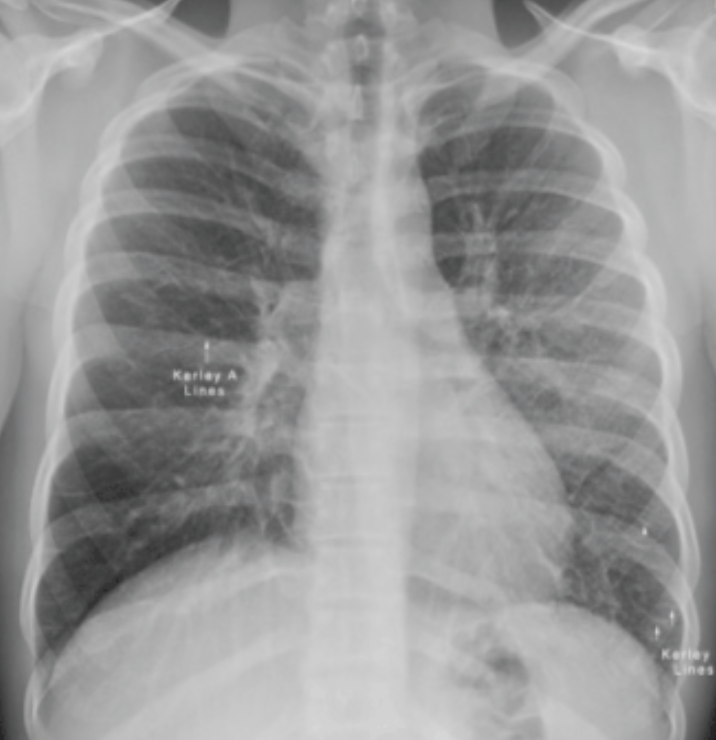
\includegraphics[width=37.76pt,height=36.44pt]{chest_x_ray.png}};

% Text Node
\draw (426,253.17) node [anchor=north west][inner sep=0.75pt]  [rotate=-89.91] [align=left] {...};
% Text Node
\draw (183.56,12.6) node [anchor=north west][inner sep=0.75pt]  [font=\large] [align=left] {{\fontfamily{pcr}\selectfont {\large Mixtures of \ Experts (MoEs)}}};
% Text Node
\draw (211.27,206.75) node [anchor=north west][inner sep=0.75pt]  [font=\LARGE]  {$fx$};
% Text Node
\draw  [draw opacity=0][fill={rgb, 255:red, 255; green, 255; blue, 255 }  ,fill opacity=0.88 ]  (174.34,252.54) -- (287.34,252.54) -- (287.34,277.54) -- (174.34,277.54) -- cycle  ;
\draw (177.34,256.54) node [anchor=north west][inner sep=0.75pt]  [font=\normalsize] [align=left] {{\fontfamily{helvet}\selectfont Gating Function}};
% Text Node
\draw    (20.28,324.95) -- (127.28,324.95) -- (127.28,349.95) -- (20.28,349.95) -- cycle  ;
\draw (23.28,328.95) node [anchor=north west][inner sep=0.75pt]  [font=\normalsize,color={rgb, 255:red, 227; green, 8; blue, 8 }  ,opacity=1 ] [align=left] {\textcolor[rgb]{0.96,0.65,0.14}{Lorem ipsum...}};
% Text Node
\draw (545.5,225.48) node [anchor=north west][inner sep=0.75pt]  [font=\large]  {$fx$};
% Text Node
\draw (305.8,109.79) node [anchor=north west][inner sep=0.75pt]  [font=\footnotesize,color={rgb, 255:red, 208; green, 2; blue, 27 }  ,opacity=1 ]  {$1.25x$};
% Text Node
\draw (303.56,189.93) node [anchor=north west][inner sep=0.75pt]  [font=\footnotesize,color={rgb, 255:red, 208; green, 2; blue, 27 }  ,opacity=1 ]  {$-2.35x$};
% Text Node
\draw (320.02,296.22) node [anchor=north west][inner sep=0.75pt]  [font=\footnotesize,color={rgb, 255:red, 208; green, 2; blue, 27 }  ,opacity=1 ]  {$0x$};
% Text Node
\draw (309.32,369.61) node [anchor=north west][inner sep=0.75pt]  [font=\footnotesize,color={rgb, 255:red, 208; green, 2; blue, 27 }  ,opacity=1 ]  {$3.46x$};
% Text Node
\draw (616.7,220.84) node [anchor=north west][inner sep=0.75pt]  [font=\Large] [align=left] {$\displaystyle \hat{y}$};


\end{tikzpicture}
        }
        \label{fig:moes}
    \end{figure}

    % Another interesting research direction would be to explore the use of MoEs to handle multimodal data. In \cite{mustafa_multimodal_2022}, researchers at Google Brain used MoEs to train an architecture that accepts both image and text inputs and outputs a single prediction by 
  
    \subsection{Meta-Learning and L2L Systems} \label{conclusions:research_directions:l2l} \info{1 pág}

    Much like human learners, who, building from previous knowledge, continuously seek and filter information that could be useful to learn new concepts and skills, an area of research in machine learning concerns the design of programs/systems that can efficiently improve their learning process without the need for explicit human intervention. This area of research is known as \textbf{meta-learning}, and it is a very active area of research in AI \todo{add citation}.
    
    Meta-learning is a technique that aims to improve the performance of machine-learning models by `learning to learn' (L2L) a certain task. Such ideas have been successfully applied to a wide range of problems, including computer vision, natural language processing, robotics, video games, and more \cite{hospedales_meta-learning_2020}.
    
    The way meta-learning is formulated is by training a model on a variety of tasks and then using the knowledge gained from those to improve its performance on new tasks or learn it faster / more sample-efficiently than if it had been trained only for that task \cite{hospedales_meta-learning_2020}.
    
    This idea is regarded to have been first introduced by Dr. Jurgen Schmidhuber in 1987 with his thesis `Evolutionary Principles in Self-Referential Learning'. In his work, Schmidhuber proposed an algorithm that adaptively improves its learning skills by recursively applying genetic programming to itself and ensuring that only `useful' modifications (made by the program to itself) `survive' in an evolutionary fashion \cite{schmidhuber_evolutionary_1987}.
    
    Recently, Finn et al. (2017) \cite{finn_model-agnostic_2017} propose a model-agnostic framework for meta-learning that can be applied to any deep-learning architecture and learning task. The framework consists of \dots

    The idea behind researching this area is that, by adopting this L2L framework, we could design a system that can continually improve its learning process over time.

    As a low-hanging fruit, we can envision the design of a system similar to the one proposed in this work that integrates and builds upon concepts from meta-learning, unlearning, knowledge distillation, and transfer learning \footnote{See section \ref{sec:relevant_techniques}}, that enables model that can more sophisticatedly adapt to new problems. 
    
    This self-adaptive process would necessarily be based on evaluating the model's performance and a metric of the `necessity' of adaptation/learning that task better, but rather than relying on simple heuristics and a model-agnostic approach, the system would trigger a more complex adaptation process.

    \clearpage
  
    % \subsection{AutoML and Neural Architecture Search} \label{conclusions:research_directions:automl_nas}

    % AutoML and Neural Architecture Search (NAS) are other two areas of research that have been gaining a lot of traction in the last few years. The idea behind these approaches is to automate the design of machine learning models by using optimization techniques to search for the best model architecture and hyperparameters for a given task.

    

    % Elisa for example tells that one could use VAEs and models like that to discover biomarkers in voxel images of lungs that could be used to evaluate the severity of the disease, discover new patterns to diagnose the disease, or find new drugs to treat it.


    \section{Final Remarks} \label{conclusions:final_remarks} \info{0.75 pág}
    
    \dots

    Unlike many scientific advances, breakthroughs such as a true self-improving model that adapts itself continually in an online fashion will have immediate applications in every domain, from healthcare to education, to economics, to scientific discovery itself \dots 

% \printbibliography
\end{document}